\documentclass[conference, 10pt]{IEEEtran}

\usepackage{cite}
\usepackage{array}
\usepackage{mdwmath}
\usepackage{mdwtab}
\usepackage[tight,footnotesize]{subfigure}
\usepackage[font=footnotesize]{subfig}
\usepackage{url}
\usepackage{comment}
\usepackage{listings}
\usepackage{graphicx}
\usepackage{multirow}
\usepackage{tabularx}

\usepackage{xspace}
\usepackage[lined]{algorithm2e}



%\renewcommand{\figurename}{\textsc{Figure}}
%\renewcommand{\thefigure}{\Roman{figure}}

% correct bad hyphenation here
\hyphenation{}

\IEEEoverridecommandlockouts

\begin{document}
%
% paper title
% can use linebreaks \\ within to get better formatting as desired
\title{Validation of a Data Center Simulation Toolkit}


% author names and affiliations
% use a multiple column layout for up to three different
% affiliations
\author{\IEEEauthorblockN{Cynric Huys\IEEEauthorrefmark{1}, Thomas Mortier\IEEEauthorrefmark{1}, Tom Naessens\IEEEauthorrefmark{1}, Jens Trogh\IEEEauthorrefmark{2}}
\IEEEauthorblockA{Computer Science: Software Engineering\IEEEauthorrefmark{1}, Electrical Engineering\IEEEauthorrefmark{2}\\ University of Ghent\\\{Cynric.Huys, ThomasF.Mortier, Tom.Naessens, Jens.Trogh\}@UGent.be}
}

% make the title area
\maketitle

\begin{abstract}
Different virtual machine allocation strategies for cloud computing systems can have a significant impact on node usage, energy consumption and SLA-achievements. DCSim is a data center simulator toolkit that, given a series of parameters, is able to simulate these different machine allocation strategies without having to execute real benchmarks. It is crucial to evaluate the accuracy of these simulated results. In this paper, DCSim is compared to an emulated cloud computing environment running OpenNebula, an open-source project delivering a feature-rich and flexible solution to build and manage clouds and virtualized data centers. By performing similar benchmarks on both the simulator and the cluster, the accuracy of precision of the simulation is assessed. When the results didn't match, some modifications were made to either the cluster or the simulator so further tests resulted in more similar results. The performed test cases are rather limited but from the gathered results, it can be concluded that for a basic set of tests and a few modifications in policies, DCSim closely matches the cluster in terms of node usage and SLA achievements. However, DCSim also sets unreal standards concerning the response time.\\
\end{abstract}

\begin{IEEEkeywords}
DCSim, cloud computing, validation, data center simulation
\end{IEEEkeywords}



\section{Introduction}

\IEEEPARstart{C}{}loud management systems nowadays are executed in huge data centers in which thousands to hundreds of thousands servers may be active. Managing these environments and making them scalable is a challenging research topic. As it is complex to evaluate such management systems, relocation policies or other algorithms on a sufficiently large scale, simulations are often used \cite{simulators}.
When the results obtained by simulation however are not sufficiently veracious, they are worthless. Hence it is crucial to analyse the correctness and accuracy of the simulation results.

Using the DCSim data center simulation toolkit \cite{6380046} and by evaluating the performance (i.e.~response time, throughput and SLA violations) of both DCSim and a physical setup, we assess the value, the usability and the reliability of the simulator when used in large scale experiments. DCSim is not too fine-grained which allows the simulation of very large experiments. Comparing the results of both the simulator and a cloud management system, it is possible to determine if the DCSim simulator is suitable for real life experiments -- i.e. if the simulator is veracious and if DCSim also acts as a real cluster when nodes are added.

First, related work is discussed in Section \ref{sec:relatedwork}. Section \ref{sec:setupandeval} describes the experimental setup of both the DCSim simulator and the emulated cloud computing environment and clarifies how both setups are evaluated. Results are listed and discussed in Section \ref{sec:results}, including the results of the first test case. This is followed by the modifications applied to our virtual and physical setup according to these first results. Section \ref{sec:conclusion} formulates the conclusion, including some final remarks. Further improvements are discussed in Section \ref{sec:futureimprovements}.


\section{Related work}
\label{sec:relatedwork}
\subsection{Application and VM placement}

When it comes to increase the performance of a cloud computing environment, allocating virtual machines (VMs) to an appropriate physical machine is very crucial \cite{cloudcomputing:allocation}. A dynamic resource allocation model based on the utilization level of physical machines in data centers is crucial since only considering a maximal use of data centers (the utilization level of physical machines in data centers) eventually has a bad influence on the performance of virtual machines (due to a high workload of each physical machine). That's why a VM allocation scheme is needed for the overall performance of cloud computing in order to prevent performance degradation.
	
Several algorithms can be compared for initial VM placement in large distributed systems \cite{VM:placementalgo}. In the research described by K.~Mills et al.~, Koala, a discrete-event simulator inspired by the Amazon Elastic Compute Cloud (EC2) and by the Eucalyptus open-source software is being used. In the experiments, VM-placement algorithms with respect to 42 response variables, grouped into six categories including user experience, cloudwide resource utilization and load, variance in cluster utilization and load, number and types of VMs and WS-message load and revenue, are being compared. 
Metrics as disk space utilization, network-interface controller loads and user request rates were also covered during the comparisons. These are important for our simulation (with the DCSim simulator) when it comes to testing the performance of our infrastructure cloud. 


The DCSim simulator uses a consolidation and relocation policy to simulate the management of virtual machines that are already running. It is therefore important to gain insight in how management policies operate \cite{datacenter:resourcemanag}.
Three policies for the continuous optimization of virtual machine placement (live migrations) can be considered: optimization over multiple system resources, network optimization and thermal optimization. These algorithms can be verified solely by simulation (using the CloudSim simulator which will be discussed in the following subsection), because of the difficulties to run a large scale experiment on a real-world infrastructure. We will verify the results of such a cloud simulator on a physical infrastructure to check its correctness.

\subsection{Simulators}
We use DCSim to simulate a data center but there are several other cloud simulators available \cite{cloudcomputing:comparison}.  All simulators have been specifically developed for performance analysis of cloud computing environments. CloudSim is the most sophisticated simulator, unlike DCSim it is not a framework with a ready to use environment for execution, instead users have to develop the cloud scenario first. CDOSim has the ability to represent the user's rather than the provider's perspective, which DCSim hasn't. TeachCloud has a simple graphical interface and is particularly made for education purposes, whereas DCSim is also suited for researchers to evaluate dynamic resource management techniques. SPECI is more focussed on analysing and exploring the scaling properties of a large data center. It is also important to mention that DCSim is designed to be easily extended to the needs of a certain research area. 

\section{Experimental setup and Evaluation}
\label{sec:setupandeval}
% explain VW and VW setup
Our aim is to assess the accuracy of DCSim compared to a real computer cluster. The UGent Virtual Wall is a complex, large scale testing facility, on which advanced network setups and data center environments can be emulated and tested \cite{virtualwall}. We are able to operate on four of its nodes, each of them having a Intel(R) Xeon(R) CPU E5620 with 16 cores, about 11.6 GiB working memory and 60 GB size capacity. Traffic between nodes is limited to 100 Mbit/second. Fig.\xspace\ref{fig:vwsetup} illustrates the Virtual Wall setup.

\begin{figure}
\centering
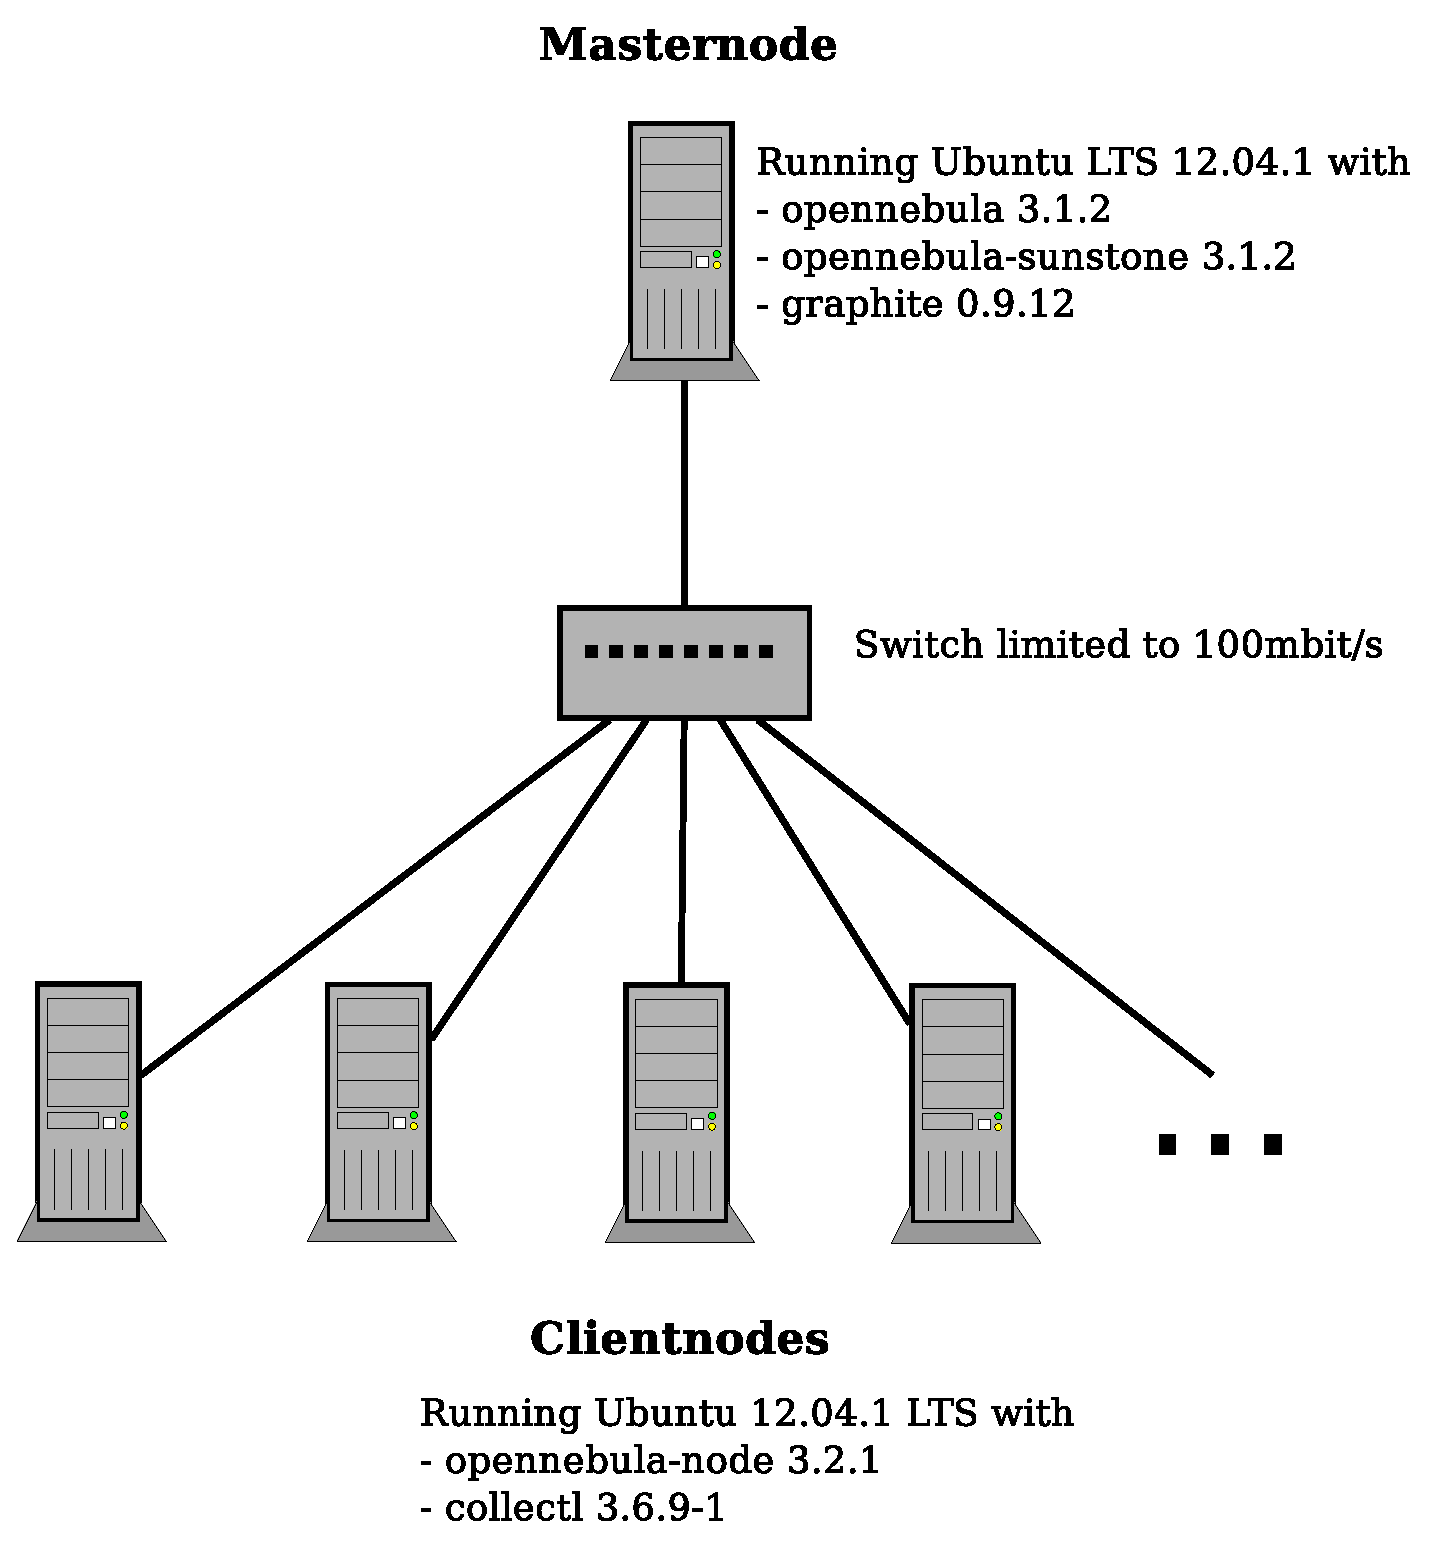
\includegraphics[width=3in]{includes/DiagramOpstelling}
\caption{Diagram representing the architecture used on the Virtual Wall.}
\label{fig:vwsetup}
\end{figure}

% OpenNebula and graphite
As the setup diagram illustrates, the stable versions of \texttt{opennebula} and \texttt{opennebula-node} were installed on the nodes. To ease monitoring and managing the virtual machines, \texttt{opennebula-sunstone} was also installed on the masternode. As the monitoring information from \texttt{opennebula-sunstone} is not very elaborate, graphite\cite{graphite} in combination with collectl \cite{collectl} was employed to monitor the workload of the individual nodes.
TTYLinux\cite{ttylinux} was used as a base image for our virtual machines as this is a very tiny, yet fully:q command-line functional, linux distribution.\\

% explain DCSim and DCSim setup
DCSim is a data center simulation toolkit based on virtual machines. The simulator offers developers and researchers a way to simulate a real data center virtual machine reallocation method in only a fraction of the actual run time of a fully fledged data center \cite{dcsim:slideshow, dcsim:paper, dcsim:paper2}. This allows researchers to determine the best virtual machine allocation pattern in a short period of time, without any overhead.

DCSim allows to configure a complete data center based on custom nodes, which we evidently based on the Virtual Wall specifications listed above. Table \ref{dcsim:vw} shows the configuration of an individual node of the Wall in the DCSim simulator. The number of CPUs, number of cores, the core capacity and memory, as well as the bandwidth and local storage is provided. A power model is included as well.\\


\begin{table}
	\renewcommand{\arraystretch}{1.3}
	\caption{Configuration of an individual node in the DCSim simulator.}
	\label{dcsim:vw}
	\begin{center}
	\tabcolsep=0.05cm
	\begin{tabularx}{3.45in}{|X|rl|rl|}
		\hline
		 \multicolumn{1}{|c|}{\multirow{2}{*}{\textbf{Parameter}}} & \multicolumn{2}{c|}{\multirow{2}{*}{\textbf{\ DCSim value\ }}} &   \multicolumn{2}{c|}{\multirow{2}{*}{\textbf{Remarks}}} \\
		&&&& \\
		\hline
		\ number of CPUs& 1 &&& \\
		\ number of cores per CPU \ & 16&&& \\
		\ CPU clock frequency& 2.400&GHz&& \\
		\ memory per CPU & 11.878 &MB& \ $\sim$ 11.6 & GiB\\
		\ bandwidth between nodes & 12.800 & kB/s \  & \ $\sim$ 100 & Mb/s \\
		\ storage capacity & \   61.440& MB & \ $\sim$ 60 & GiB \\
		\ CPU power consumption (idle state) \ &10&W& \multicolumn{2}{c|}{\cite{vw-CPU:idleusage}}\\
		\ CPU power consumption (max level) \  &80&W&\multicolumn{2}{c|}{\cite{vw-CPU:idleusage, vw-CPU:maxusage}} \\
		\hline
	\end{tabularx}
	\end{center}
\end{table}



% Algorithms
In order to assess the relative performance of both setups, a workload has to be provided. In DCSim this is done by providing a workload trace, which is used to simulate a plausible CPU load. For DCSim, a CPU trace was used that corresponds with a constant workload of $\pm100\%$. 

To emulate load on the virtual machines on the computer cluster, we ran a SPEC CPU2006\cite{spec2006} benchmark in a loop, also providing a constant CPU load of $\pm100\%$.\\

To validate the toolkit, an iterative process is followed. First, both setups are tested with their default configuration. The results from this first iteration are observed and both configurations are adopted to match one another more closely. This process gets repeated until the results match each other as close as possible or required.

First, some basic test are executed to validate the working of the simulator and the Virtual Wall. After these tests, benchmarks are executed with a fixed amount of nodes and a variable amount of virtual machines, starting at an under commitment of one virtual machine for four nodes and ending at an overcommitment of 150 virtual machines for DCSim and 100 virtual machines for the Virtual Wall.


\section{Results}
\label{sec:results}

\subsection{First results}
\subsubsection{DCSim} 
By default, DCSim applies a first fit virtual machine allocation policy \cite{firstfit}. In this first test case we evaluate the throughput, response time and SLA achievements for an increasing number of virtual machines during five hours simulation time using four nodes, configured as described in Table \ref{dcsim:vw}. Fig.\xspace\ref{fig:dcsim:throughput} illustrates the throughput for a growing number of virtual machines. The throughput remains constant, until no more virtual machines can be allocated. For DCSim, this is the case when either the number of VMs exceeds the number of cores\footnote{DCSim allows only one VM per CPU core unless we limit the available CPU power for a VM (in terms of clock frequency). This does however not fit the Virtual Wall operating mode where a VM uses all the resources available at the moment, not limited by a maximum. In this test case we use 4 nodes, each of them having a 16 core CPU.}, the accumulated storage capacity of the VMs on a particular node exceeds the node's capacity or the accumulated memory of the VMs on a particular node exceeds the node's working memory. As the nodes are configured to have a 16 core CPU, and every virtual machine is equipped with a single core CPU (Table \ref{dcsim:vm}), only 16 machines are allowed on each node.  The same behaviour is observed for both the SLA achievements (Fig.\xspace\ref{fig:dcsim:sla}) and the response time: using four nodes, each of them capable to allocate 16 virtual machines, the performance will drop as soon as the simulator tries to allocate the 65th VM\footnote{Similar scenarios occur when using more memory or storage capacity per virtual machine. If VMs were allowed to use e.g.~1 GiB, only 11 machines would be allocated per node (as a node has about 11.6 GiB working memory -- Table \ref{dcsim:vw}).}. At this point, the simulated mean response time immediately boosts to its maximum value as all available nodes are overcommitted. No more virtual machines can be allocated as none of the available nodes will be able to respond.

\begin{table}
	\renewcommand{\arraystretch}{1.3}
	\caption{Configuration of an individual virtual machine in the DCSim simulator.}
	\label{dcsim:vm}
	\begin{center}
	\tabcolsep=0.05cm
	\begin{tabular}{|l|rl|}
		\hline
		 \multicolumn{1}{|c|}{\multirow{2}{*}{\textbf{Parameter}}} & \multicolumn{2}{c|}{\multirow{2}{*}{\textbf{\ DCSim value\ }}} \\
		&& \\
		\hline
		\ number of CPUs& 1 & \\
		\ number of cores per CPU\ \ & 1& \\
		\ CPU clock frequency& 2.400&GHz\ \ \\
		\ memory& 512 &MB\\
		\ bandwidth between nodes\ \ &\ $\frac{12.800}{\tiny \textrm{\# VMs per node}}$&kB/s\\
		\ storage capacity & \  2.048& MB \\
		\ response time \ &10&ms\\
		\hline
	\end{tabular}
	\end{center}
\end{table}


\begin{figure}
\centering
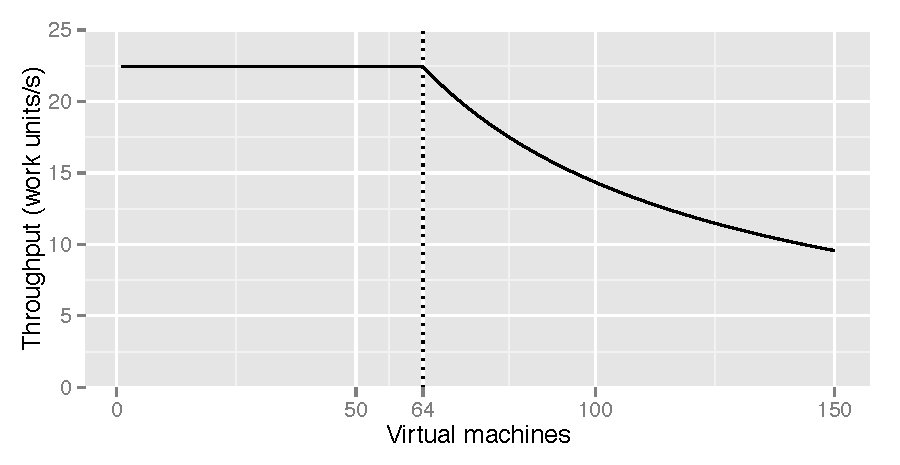
\includegraphics[width=3.4in]{includes/DCSim_throughput}
\caption{Throughput on the DCSim simulator for an increasing number of virtual machines.\protect\footnotemark}
\label{fig:dcsim:throughput}
\end{figure}

\begin{figure}
\centering
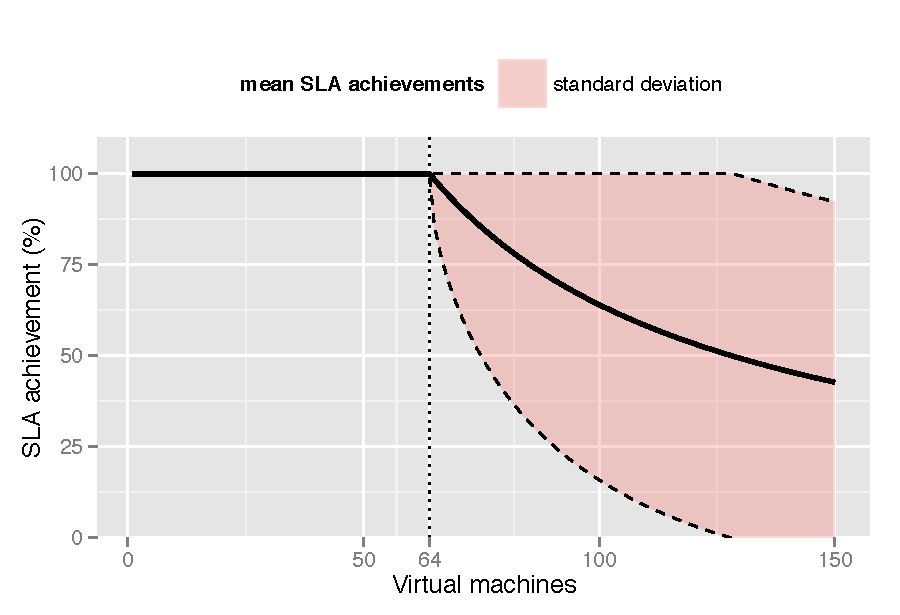
\includegraphics[width=3.4in]{includes/DCSim_SLA}
\caption{SLA achievements on the DCSim simulator for an increasing number of virtual machines.}
\label{fig:dcsim:sla}
\end{figure}


\subsubsection{Virtual Wall}
Using the default scheduler, OpenNebula tries to spread out its virtual machines over the available nodes. This effect can be seen in Fig.\xspace\ref{fig:vsm_vs_nodes}. Even if, for example, 4 virtual machines are dispatched to the processing cluster of four nodes that can perfectly fit these virtual machines next to each other on one node, OpenNebula puts each virtual machine on a different node.

Fig.\xspace\ref{fig:opennebula:responsetime} illustrates the mean response time for a number of virtual machines (in seconds). It requires time for OpenNebula to transfer and deploy a virtual image to a node. The more virtual machines are deployed, the longer this response time gets. 
The SLA achievements of the experiments can be found in Fig.\xspace\ref{fig:opennebula:sla}. The graph shows that, as long as the nodes are not overcommitted, the SLA achievement is nearly $100\%$. This SLA achievement never becomes $100\%$ as the virtual machines take a while to boot before executing their task, as explained above. From the moment the machines become overcommitted, the SLA drops significantly.
\footnotetext{A \emph{unit of work} can be interpreted freely. This can be the number of data requests, data-items to process, etc.}

\begin{figure}
\centering
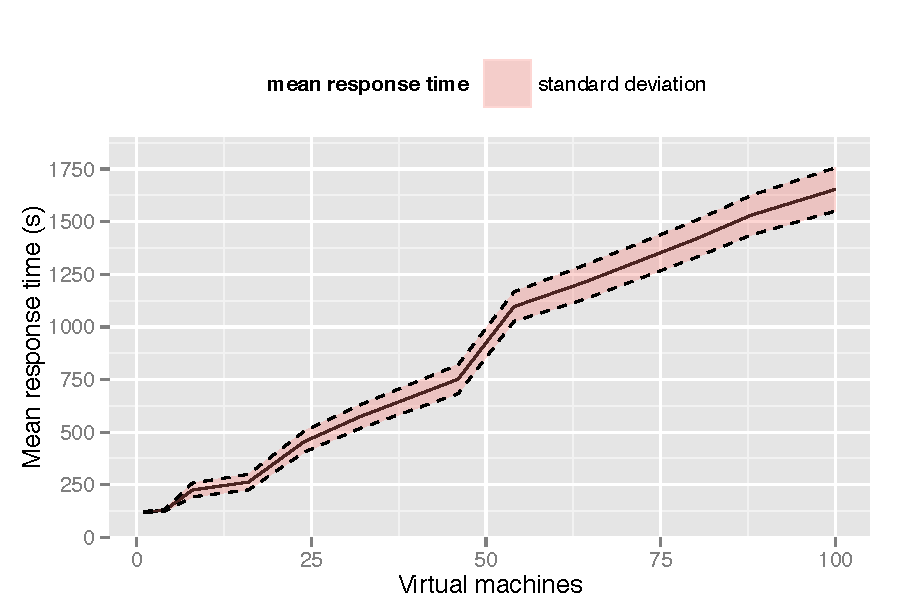
\includegraphics[width=3.4in]{includes/OpenNebula_responsetime}
\caption{The response time on the Virtual Wall for an increasing number of virtual machines.\protect\footnotemark}
\label{fig:opennebula:responsetime}
\end{figure}

\begin{figure}
\centering
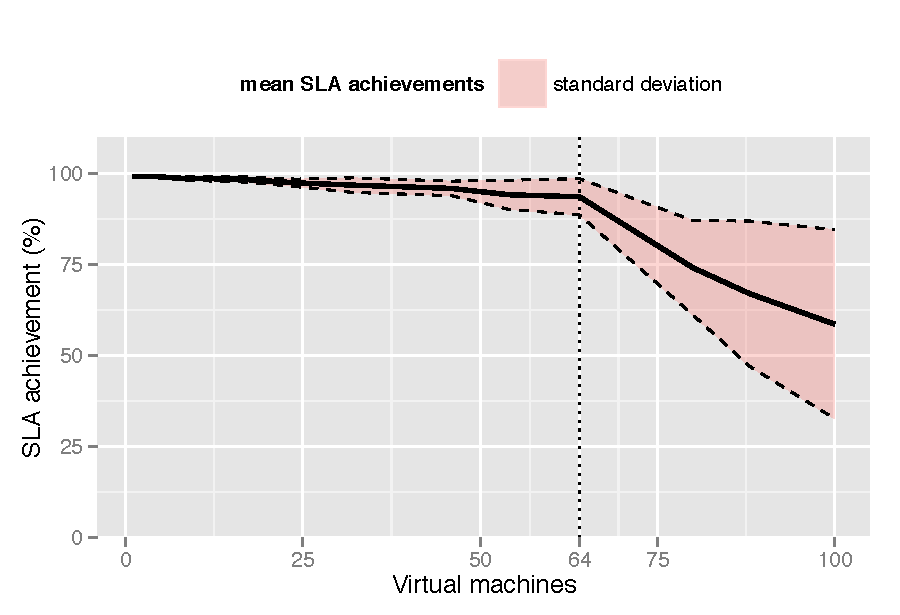
\includegraphics[width=3.4in]{includes/OpenNebula_SLA}
\caption{SLA achievements on the Virtual Wall for an increasing number of virtual machines.}
\label{fig:opennebula:sla}
\end{figure}



\subsection{Discussion}
The first noticeable difference is the number of active nodes. DCSim applies by default a first fit allocation policy while OpenNebula uses by default his own scheduler, \texttt{mm\_sched} \cite{mmsched}, which places the virtual machine on the node that has the most resources left.

Another noticeable difference is that by default, DCSim only seems to be able to host one virtual machine on each core, resulting in a maximum of 64 virtual machines for four nodes with 16 cores each. OpenNebula is able to multithread its virtual machines on one core, allowing the allocation of a (theoretically) infinite number of virtual machines; in practice however limited by the resources of the system. This results in a significant larger drop of the SLA achievements of the DCSim simulator compared to the OpenNebula cluster.
 \footnotetext{The response time can be defined as the time a host takes to be transferred to its node, to boot and to start executing tests.}

Using DCSim, the throughput metric is rather freely to interpret , it is not possible to compare the guessed estimates \emph{unit of works} with the results from the Virtual Wall. It is however expected that the throughput of the Virtuall Wall will be in line with the simulated results for a normal commitment of virtual machines. But if the nodes become over committed, DCSim just stops accepting new virtual machines, stalling the throughput. OpenNebula will however try to schedule them next to the existing virtual machine on one core, enabling some throughput instead of none.
 
Judging by the mean response time, DCSim does not take boot or transfer time into account. This is very unrealistic as a virtual machine cannot be expected to transfer, boot and start running a task instantly.

\subsection{Modifications}
\label{sec:modifications}
In order to improve the approximation of the actions and operations of a real data center, DCSim's default allocation policy should be adapted to match the OpenNebula allocation policy \emph{and} DCSim should be configured to be able to run more than one virtual machine on a CPU core. An allocation policy similar to the OpenNebula interpretation is discussed in \cite{pbf} and implemented in the DCSim simulator. Fig.\xspace\ref{fig:vsm_vs_nodes} illustrates the distribution of the virtual machines over the available nodes using the three policies. Algorithm \ref{placementPolicyVWall} briefly describes this approach.

\IncMargin{0.5em}
\begin{algorithm}
 \KwData{vmAllocationRequest}
 \KwResult{VM is placed on host with most resources left (and is capable to store this VM request)}
initialize availableHosts\;
\ForEach{Host h that is not fully utilized}{
  \If{h can host vmAllocationRequest}{
   add h to availableHosts\;
   }
 }
initialize bestHost\;
\ForEach{host h in availableHosts}{
  \If{h has more resources left than bestHost}{
	bestHost $\leftarrow$ h\;
   }
 }
allocate VM on bestHost\;
update resourcesInUse from bestHost\;
\BlankLine
\BlankLine
 \caption{DCSim allocation policy similar to OpenNebula's \texttt{mm\_sched}}
 \label{placementPolicyVWall}
\end{algorithm}
 
Using the default allocation strategy, DCSim is unable to put multiple VMs on one core. It is however possible to \emph{decrease} the virtual machine's clock frequency. In this case, the clock frequency may be considered as a share of the underlying physical CPU and hence multiple virtual machines can be assigned to a single core.
 
\begin{figure}
\centering
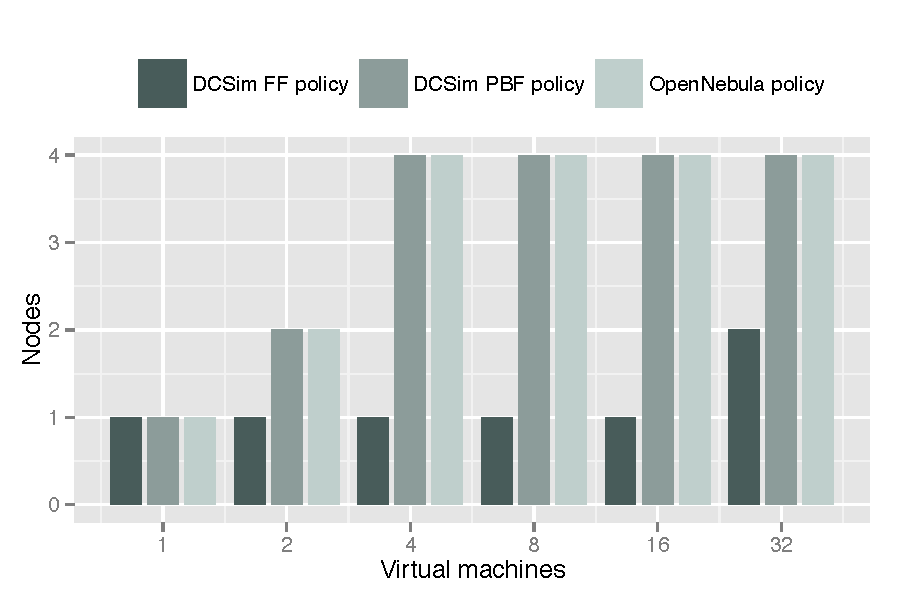
\includegraphics[width=3.4in]{includes/vms_vs_nodes}
\caption{Number of active nodes in function of the number of virtual machines using the default DCSim First Fit VM allocation policy (FF), the Power Best Fit allocation policy (PBF) and the OpenNebula default policy.}
\label{fig:vsm_vs_nodes}
\end{figure}
 
\subsection{Extended Results}
After adapting the new placement policy as shown in Algorithm\xspace\ref{placementPolicyVWall}, the amount of nodes used matches the amount of nodes OpenNebula uses perfectly, as can be seen in Fig.\xspace\ref{fig:vsm_vs_nodes}. This adaptation has however no effect on any of the other previously mentioned metrics, but does influence power consumption and power efficiency, which will not be further discussed in this paper.

\section{Conclusion}
\label{sec:conclusion}
The performed test cases are rather limited but from the results that have been gathered it can be concluded that for a basic set of tests and a few modifications in policies, DCSim closely matches the cluster in terms of node usage and SLA achievements.
When however the response time is considered, DCSim sets impossible standards of zero ms.

\section{Future Improvements}
\label{sec:futureimprovements}
When conducting the experiments on the Virtual Wall, the adopted images were stored on a local storage on the master node. This means that when a new virtual machine is created, the image needs to be transferred (using SCP, FTP, etc.) to the worker node, which is slow. It would be an improvement to create a shared storage between all nodes so the images do not have to be transferred any longer.

The previous also prevented the testing of dynamic allocation policies. The power of these policies is that virtual machines can rapidly be transferred to other,  better suited nodes. Because of the local storage, transferring images to other nodes would take too long and would result in a huge loss of performance and throughput and would increase the SLA violations.

Another improvement would of course be more extensive tests. In this project, the number of hosts remained constant. To be able to assess the correctness of DCSim, more extensive tests varying more parameters need to be performed. It would be interesting to check how well DCSim scales along with a real cluster, increasing the number of nodes and virtual machines.
\bibliographystyle{./IEEEtran}
\bibliography{./IEEEabrv,./bib}
% that's all folks
\end{document}


